\documentclass[11pt]{article}
\usepackage{graphics}
\usepackage{graphicx}
\usepackage{float}

\title{\LaTeX{} for Newbies}
\author {Anish Kumar Mishra}

\begin{document}
\maketitle

\section{Introduction}

\LaTeX{} is a typesetting program used widely in scientific community to prepare documents. It allows the user to typeset their content using tags and formatting commands.
There are several features provided by this program, some of them are typesetting, cross-referencing, embedding tables and images inside documents, etc.


\subsection{Why \LaTeX{}?} \label{ew}

A simple question one may ask that why we need yet another document preparation tool when we have so many 
of them like MS Word already available in the market. The answer to this is that \LaTeX{} comes free of cost 
and the time it takes to prepare a large document is very less. Also using \laTeX{} enables you to have more finer control over 
the appearence of your document.

\section{Getting Started}

There are some simple steps you need to follow in order to get started. It is assumed that you are trying to prepare your document on a linux system.
The steps are: 
\begin{enumerate}
  \item Open an editor of your choice(Kile or Vim).
  \item Write the following commands as shown in the figure \ref{fig1}
  \item Save the file with a .tex extension.
  \item Type the command pdflatex at your terminal.
  \item A pdf will be generated in the same folder as your .tex file.
      \begin{figure}[H]
	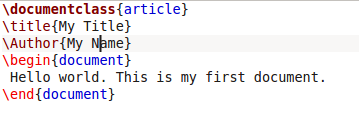
\includegraphics[width=7cm, height=3cm]{screen/shot1}
	\caption{A Simple \LaTeX{} Document}
	\label{fig1}
      \end{figure}
 \end{enumerate} 
In the above example \begin{verbatim} \documentclass, \begin, etc. \end{verbatim} 
are the commands and everything inside \verb|{..}| are the arguments to the command. 
this document will cover brief description of the commands and their usage.


\section{Document Types}

\LaTeX{} documents starts with \verb|\documentclass{class}| and end with 
\verb|\end{document}.|

\noindent Some of the well known and widely used classes are as given in table below.

\begin{table}[htb]
\caption{Document class}
\begin{tabular} {|c|l|}
\hline
{\bf Class} & {\bf Description} \\ 
\hline \hline article & for articles in scientific journals, presentations, short reports, program documentations,...\\
\hline report & for longer reports containing several chapters, small books, thesis, ... \\
\hline book & for real books \\
\hline slides & for slides \\
\hline letter & for writting letters. \\
\hline
\end{tabular}
\end{table}


\section {Inserting Pictures}
To insert a picture in your document use \verb|\begin{figure} and \end{figure}.| 
An example for this is shown below in figure\ref{fig2}.
\hspace{3mm}
\begin{figure}[H]
  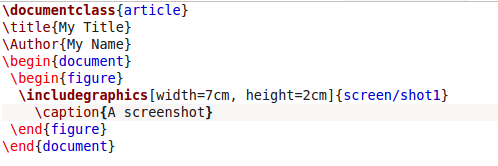
\includegraphics[width=10cm, height=3cm]{screen/shot2}
  \caption{Basic commands for figure}
  \label{fig2}
\end{figure}

Also note that you should include the package \verb|\usepackage{graphics}, \usepackage{graphicx}| 
at the beginning of your document.
\hspace{3mm}
\section {Working with Tables}
If you want a table in your document then you need to use \verb|\begin{tabular} and \end{tabular}| 
commands. 
A sample code is shown below in figure\ref{fig3}.

\begin{figure}[H]
  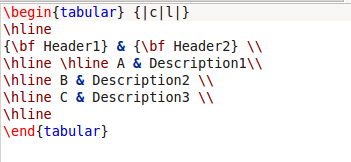
\includegraphics[width=10cm, height=3cm]{screen/shot3}
  \caption{Basic commands for table}
  \label{fig3}
\end{figure}


\end{document}